\input templates/header

\usepackage[normalem]{ulem}
\usepackage{xcolor}
\usepackage{tikz}
\usetikzlibrary{trees}
\usetikzlibrary{shapes}
\usetikzlibrary{positioning}

\newcommand*\Ball[1]{\tikz[anchor=base,baseline=-1.5pt]{
            \node[circle,ball color=blue, shade, 
 color=white,inner sep=1.2pt] (char) {\tiny #1};}}


\newcommand*\circled[1]{\tikz[baseline=(char.base)]{
            \node[minimum width=0.6cm,shape=circle,draw,inner sep=2pt,font=\ttfamily\bfseries] (char) {\small #1};}}
\newcommand*\circledr[1]{\tikz[baseline=(char.base)]{
            \node[minimum width=0.6cm,shape=circle,draw,fill=red!30,inner sep=2pt,font=\ttfamily\bfseries] (char) {\small #1};}}
\newcommand*\circledb[1]{\tikz[baseline=(char.base)]{
            \node[minimum width=0.6cm,shape=circle,draw,fill=blue!30,inner sep=2pt,font=\ttfamily\bfseries] (char) {\small #1};}}
            
\usepackage{xmpmulti}
\usepackage{listings}



\lstset{
  basicstyle=\ttfamily,
  columns=fullflexible,
  keywordstyle=\color{red}\bfseries,
  commentstyle=\color{blue},
  showstringspaces=false,
	escapeinside={(*@}{@*)},
}


\definecolor{ocra}{rgb}{1.0,0.9,0.7}
\definecolor{azzurro}{rgb}{0.8,0.8,1.0}



\title[ASD - Strutture dati]{\textbf{Algoritmi e Strutture Dati}\\[24pt]
Alberi binari di ricerca}

\graphicspath{{figs/06/}}

\begin{document}






%-------------------------------------------------------------------------
\FrameTitle{}

%-------------------------------------------------------------------------
\FrameContent

%%%%%%%%%%%%%%%%%%%%%%%%%%%%%%%%%%%%%%%%%%%%%%%%%%%%%%%%%%%%%%%%%%%%%%%%%%
\section{Alberi binari di ricerca}
%%%%%%%%%%%%%%%%%%%%%%%%%%%%%%%%%%%%%%%%%%%%%%%%%%%%%%%%%%%%%%%%%%%%%%%%%%

%-------------------------------------------------------------------------
\begin{frame}{Introduzione}

\vspace{-9pt}
\begin{myboxtitle}[Dizionario]
\EE un insieme dinamico che implementa le seguenti funzionalità:
\BIL
\item \Item \textsf{lookup}(\Item $k$)
\item \textsf{insert}(\Item $k$, \Item $v$)
\item \textsf{remove}(\Item $k$)
\EIL
\end{myboxtitle}

\begin{myboxtitle}[Possibili implementazioni]

\begin{tabular}{|l|c|c|c|}
\hline
Struttura dati & \textsf{lookup} & \textsf{insert} & \textsf{remove} \\\hline
Vettore ordinato &  $O(\log n)$ & $O(n)$ & $O(n)$ \\\hline
Vettore non ordinato &  $O(n)$ & $O(1)^*$ & $O(1)^*$ \\\hline
Lista non ordinata &  $O(n)$ & $O(1)^*$ & $O(1)^*$ \\\hline
\end{tabular}

\footnotesize
* Assumendo che l'elemento sia già stato trovato, altrimenti $O(n)$
\end{myboxtitle}

\end{frame}


%-------------------------------------------------------------------------
\begin{frame}{Alberi binari di ricerca (ABR)}


\vspace{-9pt}
\begin{myboxtitle}[Idea ispiratrice]
Portare l'idea di ricerca binaria negli alberi
\end{myboxtitle}
\TwoColsCustom{0.63}{0.35}{
\begin{myboxtitle}[Memorizzazione]
\BIL
\item Le \alert{associazioni chiave-valore} vengono memorizzate in un albero binario
\item Ogni nodo $u$ contiene una coppia ($u.\mathit{key}$, $u.\mathit{value}$)
\item Le chiavi devono appartenere ad un insieme \alert{totalmente ordinato}
\EIL
\end{myboxtitle}
}{
\begin{myboxtitle}[Nodo albero]
\vspace{-5pt}
\begin{Procedure}
\caption[A]{\textsc{Tree}}
$\Tree\ \Parentvar$\;
$\Tree\ \Leftvar$\;
$\Tree\ \Rightvar$\;
$\Item\ \mathit{key}$\;
$\Item\ \mathit{value}$\;
\end{Procedure}
\end{myboxtitle}
}

\end{frame}


%-------------------------------------------------------------------------
\begin{frame}{Alberi binari di ricerca (ABR)}

\vspace{-9pt}
\begin{myboxtitle}[Proprietà]
\BEL
\item Le chiavi contenute nei nodi del \alert{sottoalbero sinistro} di $u$ sono \alert{minori} di $u.\mathit{key}$
\item Le chiavi contenute nei  nodi del \alert{sottoalbero destro} di $u$ sono \alert{maggiori} di $u.\mathit{key}$
\EEL
\end{myboxtitle}
\TwoCols{
\vspace{-9pt}
\BB{
Le proprietà 1. e 2. permettono di realizzare un algoritmo di ricerca dicotomica
}
}{
\vspace{-12pt}
\IG{1.0}{first.pdf}
}

\end{frame}

%-------------------------------------------------------------------------
\begin{frame}{Alberi binari di ricerca -- Specifica}

\vspace{-12pt}
\TwoColsCustom{0.34}{0.6}{
\begin{myboxtitle}[Getters]
\BI
\item $\Item\ \textsf{key}()$
\item $\Item\ \textsf{value}()$	
\item $\Tree\ \textsf{left}()$
\item $\Tree\ \textsf{right}()$
\item $\Tree\ \textsf{parent}()$
\EI
\end{myboxtitle}
}{
\begin{myboxtitle}[Dizionario]
\BI
\item $\Item\ \textsf{lookup}(\Item\ k)$
\item $\textsf{insert}(\Item\ k, \Item\ v)$
\item $\textsf{remove}(\Item\ k)$
\EI
\end{myboxtitle}
}

\begin{myboxtitle}[Ordinamento]
\BI
\item $\Tree\ \textsf{successorNode}(\Tree\ t)$
\item $\Tree\ \textsf{predecessorNode}(\Tree\ t)$
\item $\Tree\ \textsf{min}()$
\item $\Tree\ \textsf{max}()$
\EI
\end{myboxtitle}


\end{frame}

%-------------------------------------------------------------------------
\begin{frame}{Alberi binari di ricerca -- Funzioni interne}

\BIL
\item \alert{$\Tree\ \lookupnode(\Tree\ T, \Item\ k)$}
\item \alert{$\Tree\ \textsf{insertNode}(\Tree\ T, \Item\ k, \Item\ v)$}
\item \alert{$\Tree\ \textsf{removeNode}(\Tree\ T, \Item\ k)$}
\EIL

\begin{Procedure}
\caption{\textsc{Dictionary}}

$\Tree\ \mathit{tree}$\;

\BlankLine
\PROCEDURE{\textsf{Dictionary}()}
{
  $\mathit{tree} = \Nil$\;
}



\end{Procedure}

\end{frame}



\subsection{Ricerca}

%-------------------------------------------------------------------------
\begin{frame}{Ricerca -- \textsf{lookupNode}()}

\vspace{-9pt}
\begin{myboxtitle}[$\Item\ \lookupnode(\Tree\ T, \Item\ k)$]
\BIL
\item Restituisce il nodo dell'albero $T$ che contiene la chiave $k$, se presente
\item Restituisce $\Nil$ se non presente
\EIL
\end{myboxtitle}

\begin{myboxtitle}[Implementazione dizionario]
\vspace{-12pt}
\begin{Procedure}
\caption[A]{$\Item\ \textsf{lookup}(\Item\ k)$}
$\Tree\ t = \lookupnode(\mathit{tree}, k)$\;
\eIf{$t \neq \Nil$}{
  \Return $t.\textsf{value}()$\;
}{
  \Return $\Nil$\;
}
\end{Procedure}
\vspace{-12pt}
\end{myboxtitle}

\end{frame}


%-------------------------------------------------------------------------
\begin{frame}{Ricerca -- esempio}

\TwoColsCustom{0.57}{0.42}{
\begin{overprint}
\includegraphics<1|handout:0>[width=\textwidth,page=2]{search-example.pdf}
\includegraphics<2|handout:0>[width=\textwidth,page=3]{search-example.pdf}
\includegraphics<3|handout:0>[width=\textwidth,page=4]{search-example.pdf}
\includegraphics<4-5|handout:1>[width=\textwidth,page=5]{search-example.pdf}
\end{overprint}
}{
\BB{Valore cercato: 3}
\BI
\item $u=\circled{6}$
\pause \item $3<6$; $u=\circled{2}$ (Sinistra)
\pause \item $3>2$; $u=\circled{4}$ (Destra)
\pause \item $3<4$; $u=\circled{3}$ (Sinistra)
\pause \item $3=3$; \alert{Trovato}
\EI
}

\end{frame}

%-------------------------------------------------------------------------
\begin{frame}{Ricerca -- Implementazione}
    
\vspace{-9pt}
\begin{myboxtitle}[Iterativa]

\begin{Procedure}
\caption[A]{\Tree \lookupnode($\Tree\ T,\ \Item\ k$)}
$\Tree\ u = T$\;
\While{$u \neq \Nil$ \AND\ $u.\Keyvar \neq k$}
{
  \eIf{$k < u.\Keyvar$}{
    $u = u.\Leftvar$\REMR{Sotto-albero di sinistra}
  }{
    $u = u.\Rightvar$\REMR{Sotto-albero di destra}
  }
}
\Return $u$\;
\end{Procedure}
\end{myboxtitle}

\end{frame}

%-------------------------------------------------------------------------
\begin{frame}{Ricerca -- esempio}

\TwoCols{
\begin{overprint}
\includegraphics<1|handout:0>[width=\textwidth,page=4]{search-example2.pdf}
\includegraphics<2|handout:1>[width=\textwidth,page=5]{search-example2.pdf}
\end{overprint}
}{
\vspace{-12pt}
\begingroup
\footnotesize
\begin{Procedure}
\caption[A]{\footnotesize \Tree \lookupnode($\Tree\ T,\ \Item\ k$)}
$\Tree\ u = T$\;
\While{$T \neq \Nil$ \AND\ $T.\Keyvar \neq k$}
{
  $u = \IIF(k < u.\Keyvar,\ u.\Leftvar,\ u.\Rightvar)$\;
}
\Return $u$\;
\end{Procedure}
\endgroup

\vspace{-12pt}
\BB{Valore cercato: 5}
\BI
\item $u=\circled{6}$
\item $5<6$; $u=\circled{2}$
\item $5>2$; $u=\circled{4}$
\item \pause $5>4$; $u=\Nil$ (Destra)
\item \Return \Nil (\alert{Non trovato})
\EI
}


\end{frame}



%-------------------------------------------------------------------------
\begin{frame}{Ricerca -- Implementazione}

\vspace{-9pt}
\begin{myboxtitle}[Ricorsiva]
\vspace{-11pt}
\begin{Procedure}
\caption[A]{\Tree \lookupnode($\Tree\ T,\ \Item\ k$)}
\eIf{$T \Eq \Nil$ \OR\ $T.\Keyvar \Eq k$}
{
  \Return $T$\;
}
{
  \Return $\lookupnode(\IIF(k < T.\Keyvar,\ T.\Leftvar,\ T.\Rightvar), k)$\;
}
\end{Procedure}
\vspace{-11pt}
\end{myboxtitle}

\end{frame}

\subsection{Minimo-massimo}


%-------------------------------------------------------------------------
\begin{frame}{Minimo-massimo}

\TwoColsCustom{0.55}{0.40}{
\includegraphics<1|handout:0>[width=\textwidth,page=1]{minmax.pdf}
\includegraphics<2|handout:0>[width=\textwidth,page=2]{minmax.pdf}
\includegraphics<3|handout:0>[width=\textwidth,page=3]{minmax.pdf}
\includegraphics<4|handout:0>[width=\textwidth,page=4]{minmax.pdf}
\includegraphics<5|handout:1>[width=\textwidth,page=5]{minmax.pdf}
}
{
\BIL
\item \texttt{min} albero radice \circled{6} ? \\
  \pause \qquad \circledr{1}

\item \texttt{max} albero radice \circled{6} ? \\
  \pause \qquad \circledr{15}

\item \texttt{max} albero radice \circled{2} ? \\
  \pause \qquad \circledr{4}

\item \texttt{min} albero radice \circled{8} ? \\
  \pause \qquad \circledr{8}
\EIL
}

\end{frame}

%-------------------------------------------------------------------------
\begin{frame}{Minimo-massimo}

\TwoColsCustom{0.55}{0.40}{
\includegraphics[width=\textwidth,page=6]{minmax.pdf}
}{
\begin{Procedure}
\caption[A]{\Tree\ \MIN(\Tree\ $T$)}
$\Tree\ u = T$\;
\While{$u.\Leftvar \neq \Nil$}{ 
  $u = u.\Leftvar$
}
\Return $u$\;

\end{Procedure}
\begin{Procedure}
\caption[A]{\Tree\ \MAX(\Tree\ $T$)}
$\Tree\ u = T$\;
\While{$u.\Rightvar \neq \Nil$}{ 
  $u = u.\Rightvar$
}
\Return $u$\;

\end{Procedure}
}

\end{frame}

%%%%%%%%%%%%%%%%%%%%%%%%%%%%%%%%%%%%%%%%%%%%%%%%%%%%%%%%%%%%%%%%%%%%%%%%%%
\subsection{Successore-predecessore}
%%%%%%%%%%%%%%%%%%%%%%%%%%%%%%%%%%%%%%%%%%%%%%%%%%%%%%%%%%%%%%%%%%%%%%%%%%

%-------------------------------------------------------------------------
\begin{frame}{Successore-predecessore -- Esempio 1}

\vspace{-9pt}
\begin{myboxtitle}[Definizione]
Il \alert{successore} di un nodo $u$ è il più piccolo nodo maggiore di $u$ 
\end{myboxtitle}

\TwoCols{
\begin{overprint}
\includegraphics<1|handout:0>[width=\textwidth,page=1]{successor.pdf}
\includegraphics<2|handout:1>[width=\textwidth,page=2]{successor.pdf}
\end{overprint}
}{
\BB{Successore di \circledr{12} ?
\onslide<2|handout:1>\circledb{15}}
}

\end{frame}

%-------------------------------------------------------------------------
\begin{frame}{Successore-predecessore -- Esempio 2}

\vspace{-9pt}
\begin{myboxtitle}[Definizione]
Il \alert{successore} di un nodo $u$ è il più piccolo nodo maggiore di $u$ 
\end{myboxtitle}

\TwoCols{
\begin{overprint}
\includegraphics<1|handout:0>[width=\textwidth,page=3]{successor.pdf}
\includegraphics<2|handout:1>[width=\textwidth,page=4]{successor.pdf}
\end{overprint}
}{
\BB{Successore di \circledr{2} ? \pause \circledb{3}}
}

\end{frame}



%-------------------------------------------------------------------------
\begin{frame}{Successore-predecessore --  Caso 1}

\vspace{-9pt}
\begin{myboxtitle}[Definizione]
Il \alert{successore} di un nodo $u$ è il più piccolo nodo maggiore di $u$ 
\end{myboxtitle}

\TwoCols{
\includegraphics[width=\textwidth,page=5]{successor.pdf}
}{
\BB{Successore di $u$?}

\pause
\begin{myboxtitle}[Caso 1]

\alert{$u$ ha figlio destro}

\bigskip
Il successore $v$ è il \alert{minimo del sottoalbero destro} di $u$
\end{myboxtitle}
}

\end{frame}

%-------------------------------------------------------------------------
\begin{frame}{Successore-predecessore -- Esempio 3}

\vspace{-9pt}
\begin{myboxtitle}[Definizione]
Il \alert{successore} di un nodo $u$ è il più piccolo nodo maggiore di $u$ 
\end{myboxtitle}

\TwoCols{
\begin{overprint}
\includegraphics<1|handout:0>[width=\textwidth,page=6]{successor.pdf}
\includegraphics<2|handout:1>[width=\textwidth,page=7]{successor.pdf}
\end{overprint}
}{
\vspace{-6pt}
\BB{Successore di \circledr{9} ? \pause \circledb{12}}
}

\end{frame}



%-------------------------------------------------------------------------
\begin{frame}{Successore-predecessore -- nodo 4}

\vspace{-9pt}
\begin{myboxtitle}[Definizione]
Il \alert{successore} di un nodo $u$ è il più piccolo nodo maggiore di $u$ 
\end{myboxtitle}

\TwoCols{
\begin{overprint}
\includegraphics<1|handout:0>[width=\textwidth,page=8]{successor.pdf}
\includegraphics<2|handout:1>[width=\textwidth,page=9]{successor.pdf}
\end{overprint}
}{
\vspace{-6pt}
\BB{Successore di \circledr{4} ? \pause \circledb{6}}
}

\end{frame}

%-------------------------------------------------------------------------
\begin{frame}{Successore-predecessore -- Caso 2}

\vspace{-9pt}
\begin{myboxtitle}[Definizione]
Il \alert{successore} di un nodo $u$ è il più piccolo nodo maggiore di $u$ 
\end{myboxtitle}

\TwoCols{
\includegraphics[width=\textwidth,page=10]{successor.pdf}
}{
\vspace{-6pt}
\BB{Successore di $u$?}

\pause
\begin{myboxtitle}[Caso 2]
\alert{$u$ non ha figlio destro}

\bigskip
Risalendo attraverso i padri, il successore è il \alert{primo avo} $v$ tale per cui $u$ sta nel \alert{sottoalbero sinistro} di $v$
\end{myboxtitle}
}

\end{frame}



%-------------------------------------------------------------------------
\begin{frame}{Successore-predecessore -- Implementazione}

\vspace{-12pt}
\TwoColsCustom{0.42}{0.56}{
\vspace{12pt}
\includegraphics[width=\textwidth,page=6]{minmax.pdf}
}{
\begin{Procedure}
\caption[A]{\Tree\ \succnode($\Tree\ t$)}

\If{$t \Eq \Nil$}{\Return $t$\;}

\uIf(\REMF{Caso 1}){$t.\Rightvar \neq \Nil$}{
  \Return $\MIN(t.\Rightvar)$\;
}
\Else(\REMF{Caso 2}){
$\Tree\ p = t.\Parentvar$\;
\While{$p \neq \Nil$ \AND\ $t \Eq p.\Rightvar$}
{
  $t = p$\;
  $p = p.\Parentvar$\;
}
\Return $p$\;
}

\end{Procedure}
}

\end{frame}

%-------------------------------------------------------------------------
\begin{frame}{Successore-predecessore -- Implementazione}

\vspace{-15pt}
\footnotesize
\TwoColsCustom{0.49}{0.49}{
\begin{Procedure}
\caption[A]{\Tree\ \alert{\prednode}($\Tree\ t$)}

\If{$t \Eq \Nil$}{\Return $t$\;}
\uIf(\REMF{Caso 1}){$t.\alert{\Leftvar} \neq \Nil$}{
  \Return $\alert{\MAX}(t.\alert{\Leftvar})$\;
}
\Else(\REMF{Caso 2}){
    $\Tree\ p = t.\Parentvar$\;
    \While{$p \neq \Nil$ \AND\ $t \Eq p.\alert{\Leftvar}$}
    {
      $t = p$\;
      $p = p.\Parentvar$\;
    }
    \Return $p$\;
}
\end{Procedure}
}{
\begin{Procedure}
\caption[A]{\Tree\ \alert{\succnode}($\Tree\ t$)}

\If{$t \Eq \Nil$}{\Return $t$\;}
\uIf(\REMF{Caso 1}){
  $t.\alert{\Rightvar} \neq \Nil$}{\Return $\alert{\MIN}(t.\alert{\Rightvar})$\;
}
\Else(\REMF{Caso 2}){
$\Tree\ p = t.\Parentvar$\;
\While{$p \neq \Nil$ \AND\ $t \Eq p.\alert{\Rightvar}$}
{
  $t = p$\;
  $p = p.\Parentvar$\;
}
\Return $p$\;
}
\end{Procedure}
}

\vspace{-9pt}
\begin{myboxtitle}[Per passare da successore a predecessore]
\BIL
\item \Rightvar diventa \Leftvar
\item \MIN\ diventa \MAX
\EIL
\end{myboxtitle}
\end{frame}


%%%%%%%%%%%%%%%%%%%%%%%%%%%%%%%%%%%%%%%%%%%%%%%%%%%%%%%%%%%%%%%%%%%%%%%%%%
\subsection{Inserimento}
%%%%%%%%%%%%%%%%%%%%%%%%%%%%%%%%%%%%%%%%%%%%%%%%%%%%%%%%%%%%%%%%%%%%%%%%%%

\begin{frame}{Inserimento -- \insertnode() }

\vspace{-9pt}
\begin{myboxtitle}[$\Tree\ \insertnode(\Tree\ T, \Item\ k, \Item\ v)$]
\BIL
\item Inserisce un'associazione chiave-valore $(k,v)$ nell'albero $T$
\item Se la chiave è già presente, sostituisce il valore associato; altrimenti, viene inserita una nuova associazione. 
\item Se $T \Eq \Nil$, restituisce il primo nodo dell'albero. 
\item Altrimenti, restituisce $T$ inalterato
\EIL
\end{myboxtitle}

\begin{myboxtitle}[Implementazione dizionario]
\vspace{-12pt}
\begin{Procedure}
\caption[A]{$\textsf{insert}(\Item\ k, \Item\ v)$}
$\mathit{tree} = \insertnode(\mathit{tree}, k, v)$\;
\end{Procedure}
\vspace{-12pt}
\end{myboxtitle}

\end{frame}

%-------------------------------------------------------------------------
\begin{frame}{Inserimento -- esempio}

\TwoColsCustom{0.57}{0.42}{
\begin{overprint}
\includegraphics<1|handout:0>[width=\textwidth,page=2]{insert-example.pdf}
\includegraphics<2|handout:0>[width=\textwidth,page=3]{insert-example.pdf}
\includegraphics<3|handout:0>[width=\textwidth,page=4]{insert-example.pdf}
\includegraphics<4|handout:1>[width=\textwidth,page=5]{insert-example.pdf}
\end{overprint}
}{
\BB{Valore da inserire: 5}
\BIL
\item $u=\circled{6}$
\pause \item $5<6$; $u=\circled{2}$ (Sinistra)
\pause \item $5>2$; $u=\circled{4}$ (Destra)
\pause \item $5>4$; $u=\Nil$ (Destra)\\ 
\alert{Inserito}
\EIL
}

\end{frame}


%-------------------------------------------------------------------------
\begin{frame}{Inserimento -- implementazione}

\vspace{-12pt}
\begin{Procedure}
\caption[A]{\Tree \insertnode($\Tree\ T,\ \Item\ k,\ \Item\ v$)}

$\Tree\ p = \Nil$\REMR{Padre}
$\Tree\ u = T$\;
\While(\REMF{Cerca posizione inserimento}){$u \neq \Nil$ \AND $u.\Keyvar \neq k$}
{
  $p = u$\;
  $u = \IIF(k < u.\Keyvar,\ u.\Leftvar,\ u.\Rightvar)$\;
}
\eIf{$u \neq \Nil$ \AND $u.\Keyvar \Eq k$}
{
  $u.\Valuevar = v$\REMR{Chiave già presente}
}
%\Else
{	
  $\Tree\ \mathit{new} = \createChild(k,v)$\REMR{Crea un nodo coppia chiave-valore}
  $\shortcut(p, \mathit{new}, k)$\;
  \If{$p \Eq \Nil$} {
    $T = \mathit{new}$\REMR{Primo nodo ad essere inserito}
  }
}
\Return $T$\REMR{Restituisce albero non modificato o nuovo nodo}
\end{Procedure}

\end{frame}

%-------------------------------------------------------------------------
\begin{frame}{Inserimento -- implementazione}


\begin{Procedure}
\caption[A]{\shortcut($\Tree\ p,\ \Tree\ u,\ \Item\ k$)}

\If{$u \neq \Nil$}{
  $u.\Parentvar = p$\REMR{Registrazione padre}
}
\If{$p \neq \Nil$}
{
  \makebox[32mm][r]{\lIf{$k < p.\Keyvar$}{}} $p.\Leftvar = u$\REMR{Attaccato come figlio sinistro}
  \makebox[32mm][r]{\lElse{}} $p.\Rightvar = u$\REMR{Attaccato come figlio destro}
}

\end{Procedure}

\end{frame}

%%%%%%%%%%%%%%%%%%%%%%%%%%%%%%%%%%%%%%%%%%%%%%%%%%%%%%%%%%%%%%%%%%%%%%%%%%
\subsection{Cancellazione}
%%%%%%%%%%%%%%%%%%%%%%%%%%%%%%%%%%%%%%%%%%%%%%%%%%%%%%%%%%%%%%%%%%%%%%%%%%

%-------------------------------------------------------------------------
\begin{frame}{Cancellazione}

\vspace{-9pt}
\begin{myboxtitle}[$\Tree\ \removenode(\Tree\ T, \Item\ k)$]
\BIL
\item Rimuove il nodo contenente la chiave $k$ dall'albero $T$
\item Restituisce la radice dell'albero (potenzialmente cambiata)
\EIL
\end{myboxtitle}

\begin{myboxtitle}[Implementazione dizionario]
\vspace{-12pt}
\begin{Procedure}
\caption[A]{$\textsf{remove}(\Item\ k)$}
$\mathit{tree} = \removenode(\mathit{tree}, k)$\;
\end{Procedure}
\vspace{-12pt}
\end{myboxtitle}


\end{frame}

%-------------------------------------------------------------------------
\begin{frame}{Cancellazione}

\TwoColsCustom{0.57}{0.42}{
\begin{overprint}
\includegraphics<1|handout:0>[width=\textwidth,page=1]{delete1.pdf}
\includegraphics<2|handout:1>[width=\textwidth,page=2]{delete1.pdf}
\end{overprint}
}{
\vspace{-12pt}
\begin{myboxtitle}[Caso 1]
\alert{Il nodo da eliminare $u$}
\alert{non ha figli}

\bigskip
Semplicemente si elimina!
\end{myboxtitle}
\begin{myboxtitle}[Esempio]
\BIL
\item Eliminazione \circledr{5}
\EIL
\end{myboxtitle}
}

\end{frame}


%-------------------------------------------------------------------------
\begin{frame}{Cancellazione}

\TwoColsCustom{0.57}{0.42}{
\begin{overprint}
\includegraphics<1|handout:0>[width=\textwidth,page=3]{delete1.pdf}
\includegraphics<2|handout:0>[width=\textwidth,page=4]{delete1.pdf}
\includegraphics<3|handout:1>[width=\textwidth,page=5]{delete1.pdf}
\end{overprint}
}{
\vspace{-12pt}
\begin{myboxtitle}[Caso 2]
\alert{Il nodo da eliminare $u$}
\alert{ha un solo figlio $f$}

\bigskip
Si elimina $u$

\bigskip
Si attacca $f$ all'ex-padre $p$ di $u$ in sostituzione di $u$ 
(\alert{short-cut})
\end{myboxtitle}
\begin{myboxtitle}[Esempio]
\BIL
\item Eliminazione \circledr{4}
\EIL
\end{myboxtitle}
}

\end{frame}

%-------------------------------------------------------------------------
\begin{frame}{Cancellazione}

\begin{overprint}
\onslide<1|handout:1>
\begin{center} 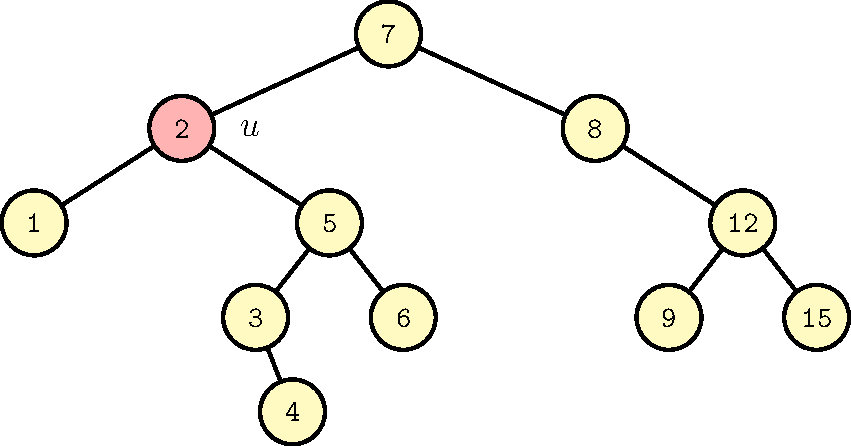
\includegraphics[width=0.8\textwidth,page=1]{delete2.pdf} \end{center}
\onslide<2|handout:2>
\begin{center} \includegraphics[width=0.8\textwidth,page=2]{delete2.pdf} \end{center}
\onslide<3|handout:3>
\begin{center} \includegraphics[width=0.8\textwidth,page=3]{delete2.pdf} \end{center}
\onslide<4|handout:4>
\begin{center} \includegraphics[width=0.8\textwidth,page=4]{delete2.pdf} \end{center}
\onslide<5|handout:5>
\begin{center} \includegraphics[width=0.8\textwidth,page=5]{delete2.pdf} \end{center}
\end{overprint}

\vspace{-12pt}
\begin{myboxtitle}[Caso 3]
\begin{overprint}
\onslide<1|handout:1>
\alert{Il nodo da eliminare $u$ ha due figli}
\BIL
\item Eliminazione \circledr{2}
\EIL

\onslide<2|handout:2>
\BIL
\item Si individua il successore $s$ di $u$
\item Il successore non ha figlio sinistro
\EIL
\onslide<3|handout:3>
\BIL
\item Si “stacca” il successore
\EIL
\onslide<4|handout:4>
\BIL
\item Si attacca l'eventuale figlio destro di $s$ al padre di $s$ (\alert{short-cut})
\EIL
\onslide<5|handout:5>
\BIL
\item Si copia $s$ su $u$
\item Si rimuove il nodo $s$
\EIL
\end{overprint}
\end{myboxtitle}
% \begin{myboxtitle}[Esempio]
% \BIL
% \item Eliminazione \circledr{2}
% \EIL
% \end{myboxtitle}

\end{frame}

%-------------------------------------------------------------------------
\begin{frame}{Cancellazione -- Implementazione}

\footnotesize
\vspace{-12pt}
\begin{Procedure}
\caption[A]{\Tree\ \removenode($\Tree\ T,\ \Item\ k$)}

$\Tree\ t$\;
$\Tree\ u = \lookupnode(T, k)$\;
\If{$u \neq \Nil$} {
\uIf(\REMF{Caso 1}){$u.\Leftvar \Eq \Nil$ \AND\ $u.\Rightvar \Eq \Nil$}{
  $\shortcut(u.\Parentvar, \Nil, k)$\;
  \DELETE $u$\;
}
\uElseIf(\REMF{Caso 3}){$u.\Leftvar \neq \Nil$ \AND\ $u.\Rightvar \neq \Nil$}
{
  [...]\;
}
\Else(\REMF{Caso 2}){
  [...]\;
}
}
\Return $T$\;
\end{Procedure}

\end{frame}

%-------------------------------------------------------------------------
\begin{frame}{Cancellazione -- Implementazione}

\footnotesize
\vspace{-12pt}
\begin{Procedure}
\caption[A]{\Tree\ \removenode($\Tree\ T,\ \Item\ k$)}

$\Tree\ t$\;
$\Tree\ u = \lookupnode(T, k)$\;
\If{$u \neq \Nil$} {
\uIf(\REMF{Caso 1}){$u.\Leftvar \Eq \Nil$ \AND\ $u.\Rightvar \Eq \Nil$}{
  [...]\;
}
\uElseIf(\REMF{Caso 3}){$u.\Leftvar \neq \Nil$ \AND\ $u.\Rightvar \neq \Nil$}
{
  $\Tree\ s = \succnode()$\;
  $\shortcut(s.\Parentvar, s.\Rightvar, s.\Keyvar)$\;
  $u.\Keyvar = s.\Keyvar$\;
  $u.\Valuevar = s.\Valuevar$\;
  \DELETE $s$\;    
}
\Else(\REMF{Caso 2}){
  [...]\;
}
}
\Return $T$\;
\end{Procedure}

\end{frame}

%-------------------------------------------------------------------------
\begin{frame}{Cancellazione -- Implementazione}

\footnotesize
\vspace{-12pt}
\begin{Procedure}
\caption[A]{\Tree\ \removenode($\Tree\ T,\ \Item\ k$)}

$\Tree\ t$\;
$\Tree\ u = \lookupnode(T, k)$\;
\If{$u \neq \Nil$} {
\uIf(\REMF{Caso 1}){$u.\Leftvar \Eq \Nil$ \AND\ $u.\Rightvar \Eq \Nil$}{
  [...]\;
}
\uElseIf(\REMF{Caso 3}){$u.\Leftvar \neq \Nil$ \AND\ $u.\Rightvar \neq \Nil$}
{
  [...]\;
}
\uElseIf(\REMF{Caso 2}){$u.\Leftvar \neq \Nil$ \AND\ $u.\Rightvar \Eq \Nil$}{
  $\shortcut(u.\Parentvar, u.\Leftvar, k)$\; 
  \If{$u.\Parentvar = \Nil$}{$T = u.\Leftvar$}
}
\Else{
  $\shortcut(u.\Parentvar, u.\Rightvar, k)$\;
  \If{$u.\Parentvar = \Nil$}{$T = u.\Rightvar$}
}
}
\Return $T$\;
\end{Procedure}

\end{frame}

\begin{frame}{Cancellazione -- Dimostrazione}

\vspace{-9pt}
\begin{myboxtitle}[Caso 1 - nessun figlio]
\BI
\item Eliminare foglie non cambia l'ordine dei nodi rimanenti
\EI
\end{myboxtitle}
\begin{myboxtitle}[Caso 2 - solo un figlio (destro o sinistro)]
\BI
\item Se $u$ è il figlio destro (sinistro) di $p$, tutti i valori nel sottoalbero di $f$ sono maggiori (minori) di $p$
\item Quindi $f$ può essere attaccato come figlio destro (sinistro) di $p$ al posto di $u$
\EI
\end{myboxtitle}

\end{frame}

\begin{frame}{Cancellazione -- Dimostrazione}

\vspace{-9pt}
\begin{myboxtitle}[Caso 3 - due figli]
\BI
\item Il successore $s$ 
\BI
\item è sicuramente $\geq$ dei nodi nel sottoalbero sinistro di $u$
\item è sicuramente $\leq$ dei nodi nel sottoalbero destro di $u$
\EI
\item quindi può essere sostituito a $u$
\item A quel punto, si ricade nel caso $2$
\EI
\end{myboxtitle}

\end{frame}


%%%%%%%%%%%%%%%%%%%%%%%%%%%%%%%%%%%%%%%%%%%%%%%%%%%%%%%%%%%%%%%%%%%%%%%%%%
\subsection{Costo computazionale}
%%%%%%%%%%%%%%%%%%%%%%%%%%%%%%%%%%%%%%%%%%%%%%%%%%%%%%%%%%%%%%%%%%%%%%%%%%

%-------------------------------------------------------------------------
\begin{frame}{Costo computazionale}

\vspace{-12pt}
\TwoCols{
\begin{myboxtitle}[Osservazione]
Tutte le operazioni sono confinate ai nodi posizionati lungo un cammino semplice 
dalla radice ad una foglia

\bigskip
$h = \textrm{\alert{Altezza dell'albero}}$

\bigskip
Tempo di ricerca: $O(h)$
\end{myboxtitle}

\begin{myboxtitle}[Domande]
\BIL
\item Qual è il caso pessimo?
\item Qual è il caso ottimo?
\EIL
\end{myboxtitle}
}{
\begin{myboxtitle}[Esempio]
\IG{1.0}{height.pdf}
\end{myboxtitle}
}

\end{frame}

%-------------------------------------------------------------------------
\begin{frame}{Costo computazionale}

\vspace{-12pt}
\TwoCols{
\begin{myboxtitle}[Osservazione]
Le operazioni di ricerca sono confinate ai nodi posizionati lungo un cammino semplice 
dalla radice ad una foglia

\bigskip
$h = \textrm{\alert{Altezza dell'albero}}$

\bigskip
Tempo di ricerca: $O(h)$
\end{myboxtitle}

\begin{myboxtitle}[Domande]
\BIL
\item Qual è il caso pessimo?
\item Qual è il caso ottimo?
\EIL
\end{myboxtitle}
}{
\begin{myboxtitle}[Caso pessimo: $h = O(n)$]
\IG{0.39}{pessimo.pdf}
\end{myboxtitle}
}

\end{frame}


%-------------------------------------------------------------------------
\begin{frame}{Costo computazionale}

\vspace{-12pt}
\TwoCols{
\begin{myboxtitle}[Osservazione]
Le operazioni descritte sono confinate ai nodi posizionati lungo un cammino semplice 
dalla radice ad una foglia

\bigskip
$h = \textrm{\alert{Altezza dell'albero}}$

\bigskip
Tempo di ricerca: $O(h)$
\end{myboxtitle}

\begin{myboxtitle}[Domande]
\BIL
\item Qual è il caso pessimo?
\item Qual è il caso ottimo?
\EIL
\end{myboxtitle}
}{
\begin{myboxtitle}[Caso ottimo: $h = O(\log n)$]
\IG{1.0}{first.pdf}
\end{myboxtitle}
}
\end{frame}

%-------------------------------------------------------------------------
\title[ASD - Strutture dati]{\textbf{Algoritmi e Strutture Dati}\\[24pt]
Alberi binari di ricerca bilanciati}
\FrameTitle{}

%-------------------------------------------------------------------------
\section{Alberi binari di ricerca bilanciati}

\begin{frame}{Altezza degli alberi binari di ricerca}

\vspace{-9pt}
\begin{myboxtitle}[Altezza ABR, caso pessimo]
\BIL
\item $O(n)$
\EIL	
\end{myboxtitle}

\begin{myboxtitle}[Altezza ABR, caso medio]
\BIL
\item Caso "semplice": inserimenti in ordine casuale
  \BI
  \item \EE possibile dimostrare che l'altezza media è $O(\log n)$
  \EI
\item Caso generale (inserimenti + cancellazioni): 
  \BI
  \item Difficile da trattare
  \EI
\EIL
\end{myboxtitle}


\begin{myboxtitle}[Nella realtà]
\BIL
\item Non ci si affida al caso
\item Si utilizzano tecniche per mantenere l'albero bilanciato
\EIL
\end{myboxtitle}

\end{frame}

%-------------------------------------------------------------------------
\begin{frame}{ABR bilanciati}

\vspace{-9pt}
\begin{myboxtitle}[Fattore di bilanciamento]
Il \alert{fattore di bilanciamento} $\beta(v)$ di un nodo $v$ è la massima differenza di altezza fra i sottoalberi di $v$
\end{myboxtitle}

\BIL
\item \alert{Alberi AVL} (Adelson-Velskii e Landis, 1962)
\BI
\item $\beta(v) \leq 1$  per ogni nodo $v$
\item Bilanciamento ottenuto tramite \alert{rotazioni}
\EI
\item \alert{B-Alberi} (Bayer, McCreight,  1972)
\BI
\item $\beta(v) = 0$ per ogni nodo $v$
\item  Specializzati per strutture in memoria secondaria
\EI
\item \alert{Alberi 2-3} (Hopcroft, 1983)
\BI
\item  $\beta(v) = 0$ per ogni nodo $v$
\item Bilanciamento ottenuto tramite \alert{merge/split}, grado variabile
\EI
\EIL

\end{frame}

\subsection{Definizioni}

%-------------------------------------------------------------------------
\begin{frame}{Alberi Red-Black (Guibas and Sedgewick, 1978)}

\vspace{-9pt}
\BB{
Sono \alert{alberi binari di ricerca} in cui:
\BIL
\item Ogni nodo è colorato di \alert{rosso} o di \alert{nero}
\item Le \alert{chiavi} vengono mantenute \alert{solo nei nodi interni} dell'albero
\item Le foglie sono costituite da \alert{nodi speciali \textbf{Nil}} 
\item Vengono rispettati i seguenti vincoli:
\BEL
\item La radice è nera
\item Tutte le foglie sono nere
\item Entrambi i figli di un nodo rosso sono neri
\item Ogni cammino semplice da un nodo $u$ ad una delle foglie contenute nel suo sottoalbero ha lo stesso numero di nodi neri
\EEL
\EIL
}

\end{frame}

%-------------------------------------------------------------------------
\begin{frame}{Esempi}

\vspace{-12pt}
\begin{overprint}

\onslide<1|handout:1>
\BB{\Ball{1} La radice è nera}

\onslide<2|handout:2>
\BB{\Ball{2} Tutte le foglie sono nere}

\onslide<3|handout:3>
\BB{\Ball{3} Entrambi i figli di un nodo rosso sono neri}

\onslide<4|handout:4>
\BB{\Ball{4} Ogni cammino semplice da un nodo $u$ ad una delle foglie contenute nel suo sottoalbero ha lo stesso numero di nodi neri }

\end{overprint}

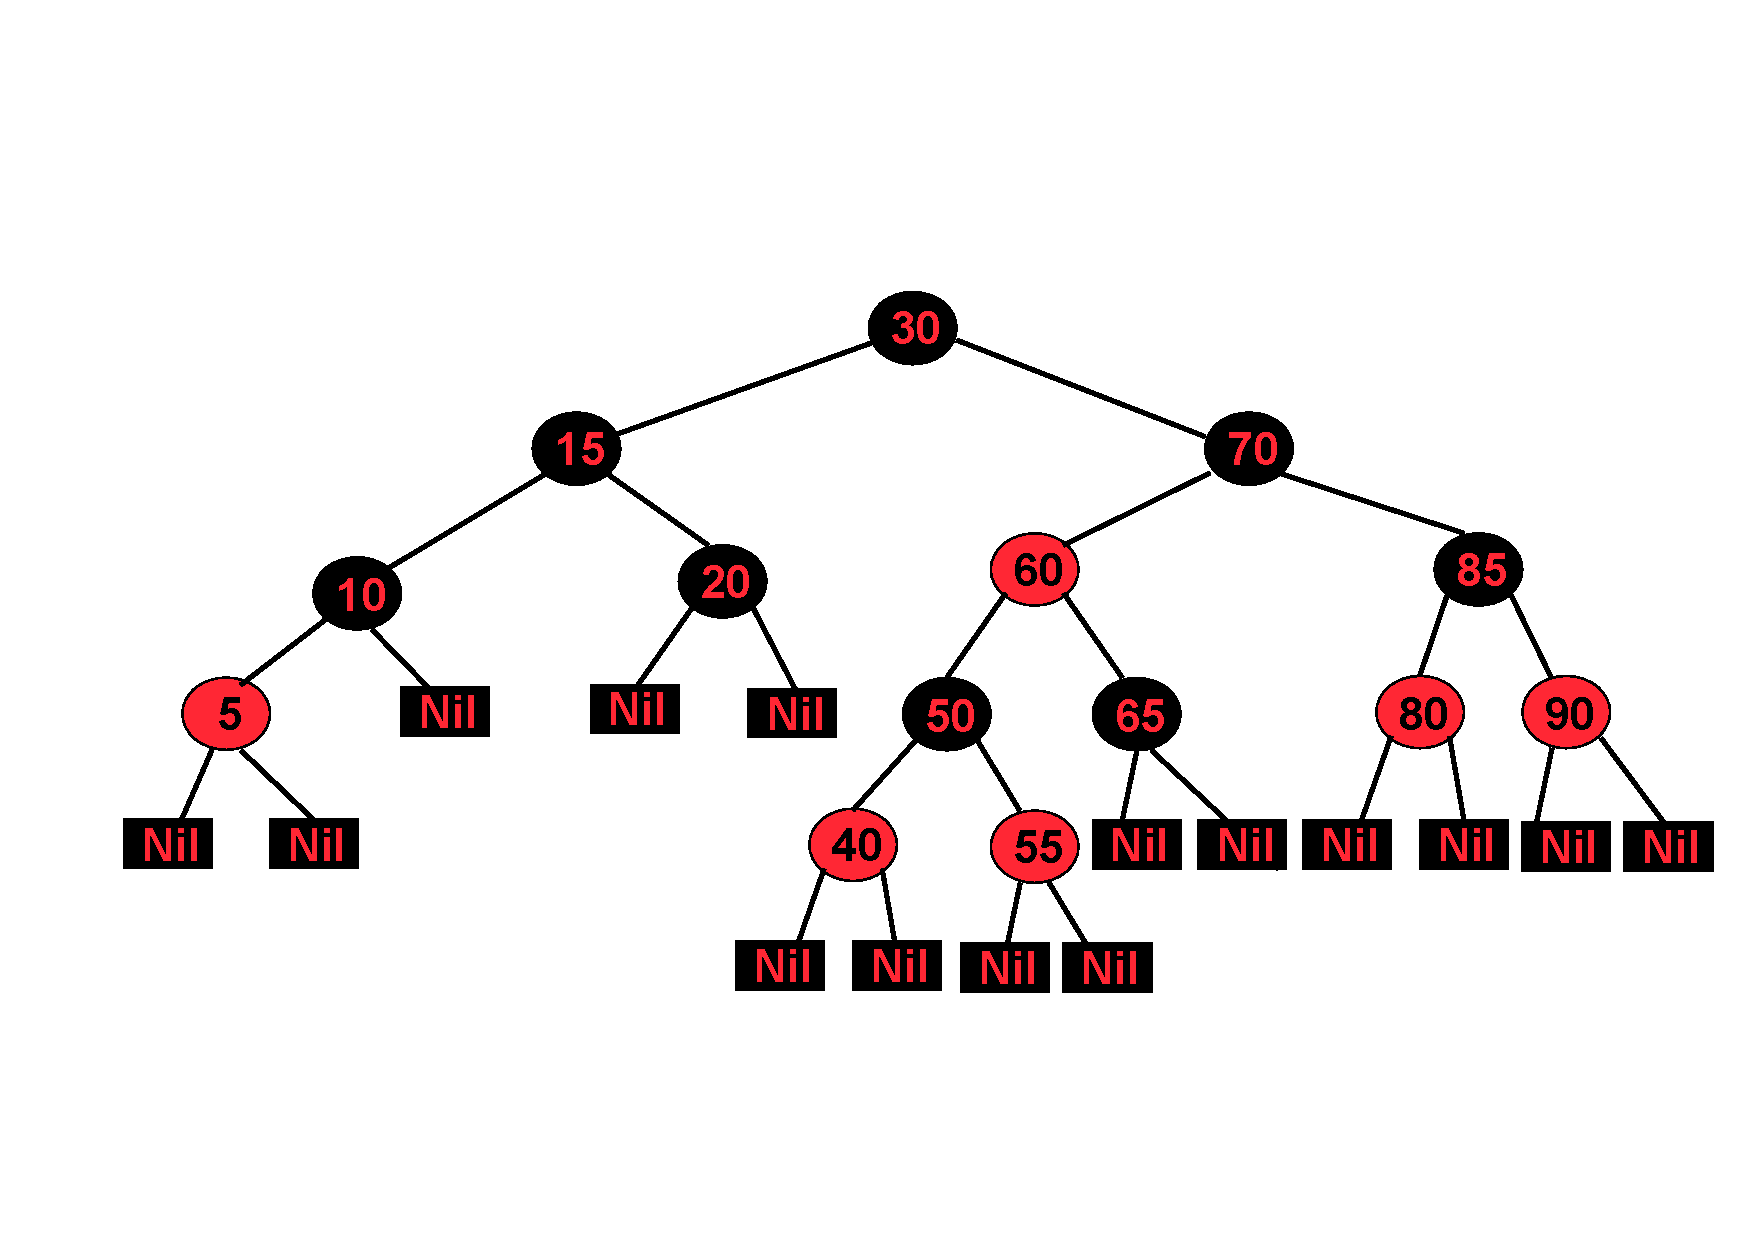
\includegraphics[width=1.0\textwidth,page=1]{redblack1.pdf}

\end{frame}

%-------------------------------------------------------------------------
\begin{frame}{Reality check}

\vspace{-9pt}
\begin{myboxtitle}[Java TreeMap, Java TreeSet]
\tiny
\url{https://docs.oracle.com/javase/8/docs/api/java/util/TreeMap.html}

\smallskip
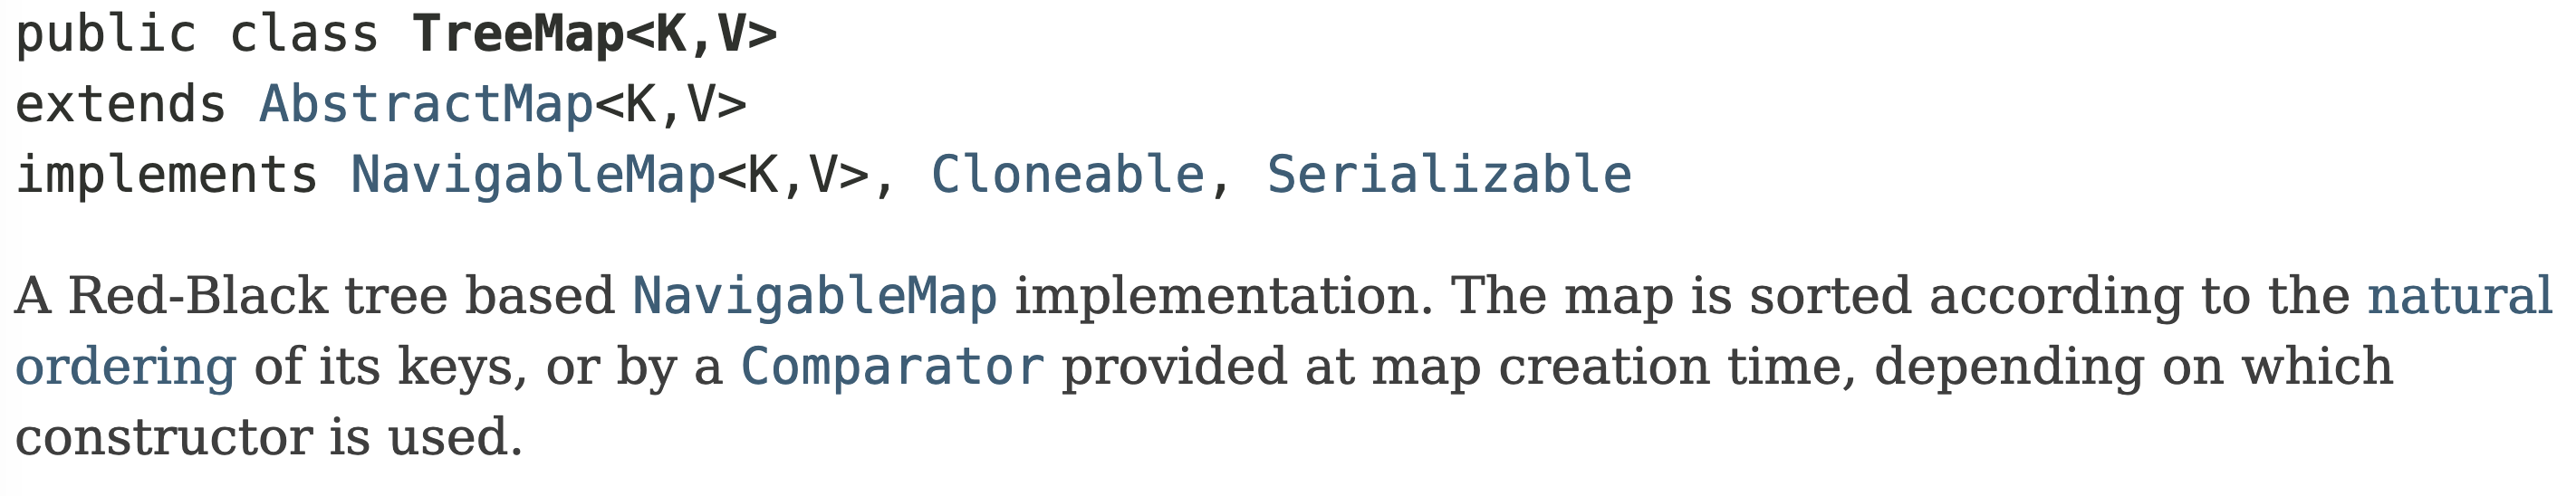
\includegraphics[width=\linewidth]{treemap.png}
\vspace{-9pt}
\end{myboxtitle}

\begin{myboxtitle}[C++ STL]
\tiny
\url{https://gcc.gnu.org/onlinedocs/libstdc++/libstdc++-html-USERS-4.1/stl__tree_8h-source.html}

\smallskip
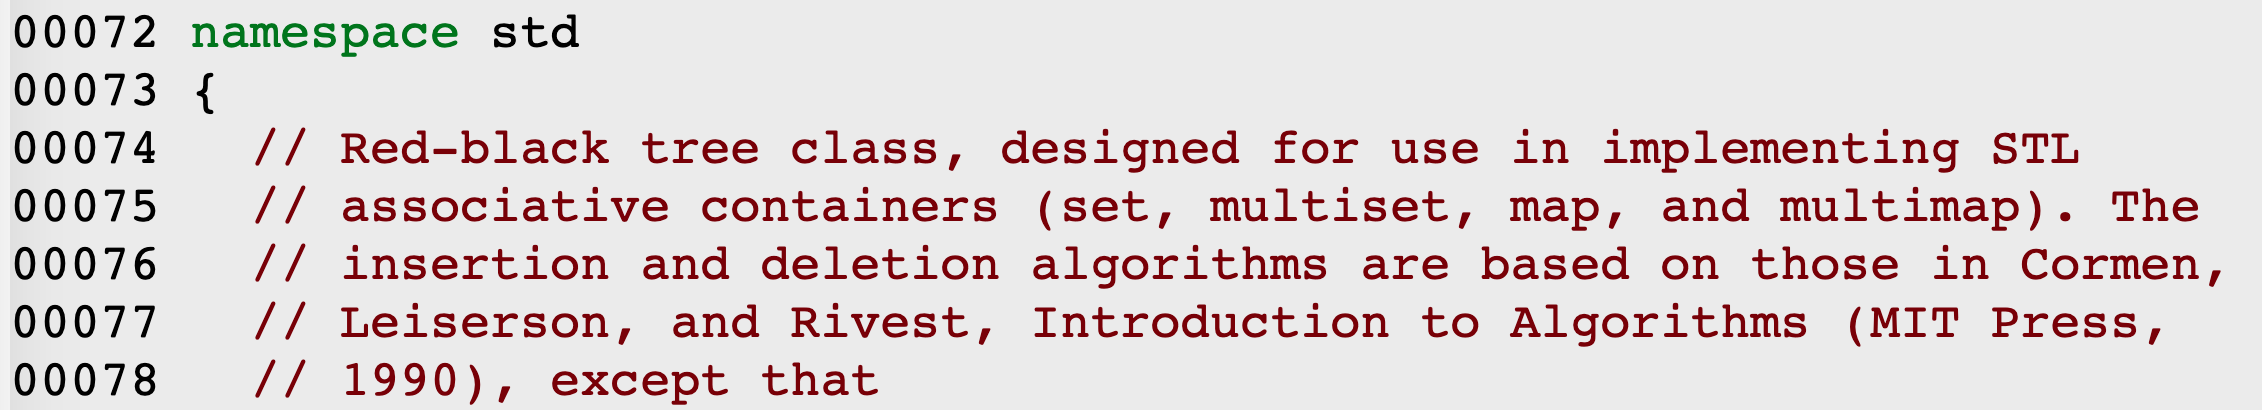
\includegraphics[width=\linewidth]{stl.png}
\vspace{-9pt}
\end{myboxtitle}

\end{frame}


%-------------------------------------------------------------------------
\begin{frame}{Reality check}

\vspace{-9pt}
\begin{myboxtitle}[Linux]
\tiny
\url{https://github.com/torvalds/linux/blob/master/Documentation/core-api/rbtree.rst}

\smallskip
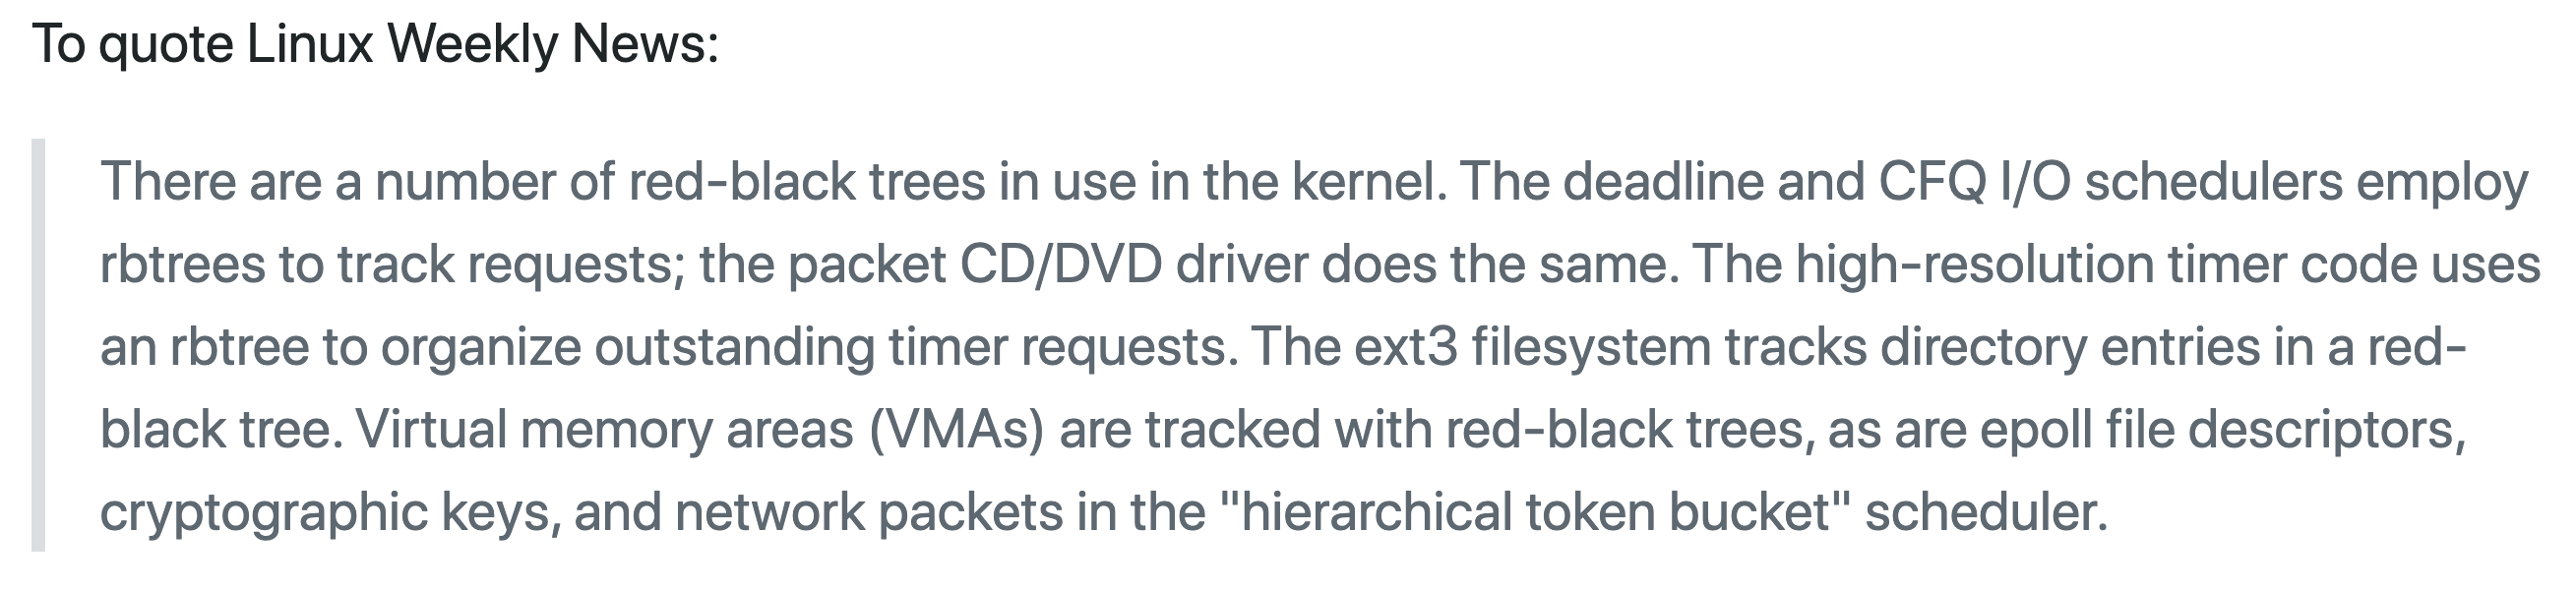
\includegraphics[width=1.0\linewidth]{linux2.png}

\smallskip
\url{https://github.com/torvalds/linux/blob/master/include/linux/rbtree.h}

\smallskip

\includegraphics[width=1.0\linewidth]{linux3.png}
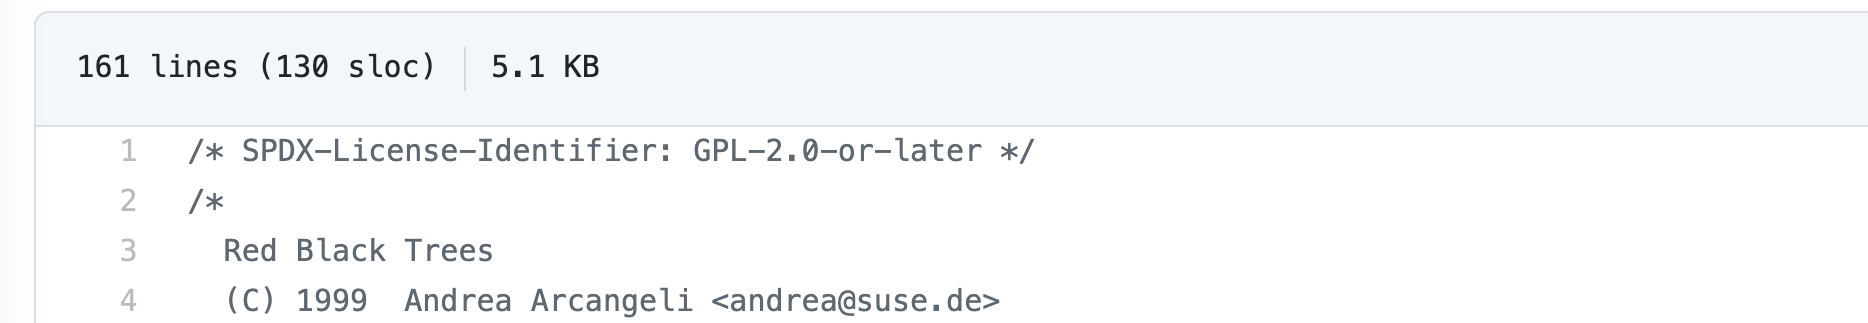
\includegraphics[width=1.0\linewidth]{linux4.png}
\end{myboxtitle}

\end{frame}


%-------------------------------------------------------------------------
\begin{frame}{Alberi Red-Black -- Memorizzazione}

\TwoColsCustom{0.30}{0.65}{
\begin{Procedure}
\caption[A]{\textsc{Tree}}
$\Tree\ \Parentvar$\;
$\Tree\ \Leftvar$\;
$\Tree\ \Rightvar$\;
$ \alert{\INTEGER\ \mathit{color}}$\;
$\Item\ \mathit{key}$\;
$\Item\ \mathit{value}$\;
\end{Procedure}
}{
\begin{myboxtitle}[Nodi \textbf{Nil}]
\BIL
\item Nodo \alert{sentinella} il cui scopo è avere accesso al colore di entrambi i figli, evitare di dover gestire casi particolari quando uno dei due è \Nil.
\item Al posto di un puntatore \Nil, si usa un puntatore ad un nodo \textbf{Nil} con colore nero
\item Ne esiste solo uno, per risparmiare memoria
\EIL
\end{myboxtitle}
}
\end{frame}

%-------------------------------------------------------------------------
\begin{frame}{Altezza nera}

\vspace{-9pt}
\begin{myboxtitle}[Altezza nera di un nodo $v$]
L'\alert{altezza nera $\mathit{bh}(v)$ di un nodo $v$} è il numero di nodi neri lungo ogni cammino da $v$ (escluso) ad ogni foglia (inclusa) del suo sottoalbero.
\end{myboxtitle}

\begin{myboxtitle}[Altezza nera di un albero Red-Black]
L'\alert{altezza nera di un albero Red-Black} è pari all'altezza nera della sua radice
\end{myboxtitle}


\vspace{48pt}
\hrule

\vspace{6pt}
Entrambe ben definite perché tutti i cammini hanno lo stesso numero di nodi neri (Vincolo (4))

\end{frame}

\subsection{Esempi}

%-------------------------------------------------------------------------
\begin{frame}{Esempi}

\vspace{-12pt}
\begin{overprint}

\onslide<1|handout:1>
\BB{Più colorazioni sono possibili -- Versione 1\\
Altezza nera: \alert{$\mathit{bh}(r)=3$}}

\onslide<2|handout:2>
\BB{Più colorazioni sono possibili -- Versione 2\\
Altezza nera: \alert{$\mathit{bh}(r)=3$}}

\onslide<3|handout:3>
\BB{Cambiare colorazione può cambiare l'altezza nera\\
Altezza nera: \alert{$\mathit{bh}(r)=3$}}

\onslide<4|handout:4>
\BB{Cambiare colorazione può cambiare l'altezza nera\\ 
Altezza nera: \alert{$\mathit{bh}(r)=2$}}

\onslide<5|handout:5>
\BB{Questo albero può essere un albero Red-Black?\\}

\onslide<6|handout:6>
\BB{Guardando il lato sinistro, $2 \leq \mathit{bh}(r) \leq 3$\\
Guardando il lato destro, $\mathit{bh}(r) \geq 3$\\
Quindi \alert{bh(r)=3}.
}


\onslide<7|handout:7>
\BB{Supponiamo che 60 e 70 siano entrambi neri.\\
\alert{Per rispettare il vincolo \Ball{4}, dobbiamo infrangere il vincolo \Ball{3}}
}

% \onslide<8|handout:8>
% \BB{Quindi, almeno uno fra 60 e 70 deve essere rosso.\\
% Per il vincolo 3, al massimo uno fra 60 e 70 deve essere rosso.}


\onslide<8|handout:8>
\BB{Proviamo a colorare di  rosso il nodo 60.\\ 
Esistono cammini con 2 nodi neri e con 3 nodi neri.\\ 
\alert{Impossibile per il vincolo \Ball{4}}}

\onslide<9|handout:9>
\BB{Proviamo a colorare di rosso il nodo 70.\\
Esistono cammini con 2 nodi neri\\
\alert{Impossibile per il vincolo \Ball{4}}
}

\onslide<10|handout:10>
\BB{Questa è l'ultima possibilità.\\
\alert{Impossibile perchè non rispetta il vincolo \Ball{1}}\\
\alert{Impossibile perchè non rispetta il vincolo \Ball{4}}
}

\onslide<11|handout:11>
\BB{Questo albero non può essere un albero Red-Black!
}

\end{overprint}

\begin{overprint}
\includegraphics<1|handout:1>[width=1.0\textwidth,page=3]{redblack1.pdf}
\includegraphics<2|handout:2>[width=1.0\textwidth,page=4]{redblack1.pdf}
\includegraphics<3|handout:3>[width=1.0\textwidth,page=5]{redblack1.pdf}
\includegraphics<4|handout:4>[width=1.0\textwidth,page=6]{redblack1.pdf}
\includegraphics<5|handout:5>[width=1.0\textwidth,page=7]{redblack1.pdf}
\includegraphics<6|handout:6>[width=1.0\textwidth,page=7]{redblack1.pdf}
\includegraphics<7|handout:7>[width=1.0\textwidth,page=9]{redblack1.pdf}
%\includegraphics<8|handout:8>[width=1.0\textwidth,page=10]{redblack1.pdf}
\includegraphics<8|handout:8>[width=1.0\textwidth,page=11]{redblack1.pdf}
\includegraphics<9|handout:9>[width=1.0\textwidth,page=12]{redblack1.pdf}
\includegraphics<10|handout:10>[width=1.0\textwidth,page=13]{redblack1.pdf}
\includegraphics<11|handout:11>[width=1.0\textwidth,page=14]{redblack1.pdf}
\end{overprint}

\end{frame}

\subsection{Inserimento}


%-------------------------------------------------------------------------
\begin{frame}{Inserimento}

\BB{Durante la modifica di un albero Red-Black}
\BIL
\item \EE possibile che le condizioni di bilanciamento risultino violate
\EIL
\BB{Quando i vincoli Red-Black vengono violati si può agire:}
\BIL
\item Modificando i colori nella zona della violazione
\item Operando dei ribilanciamenti dell’albero tramite \alert{rotazioni}
  \BI
  \item \alert{Rotazione destra}
  \item \alert{Rotazione sinistra}
  \EI
\EIL

\end{frame}

%-------------------------------------------------------------------------
\begin{frame}{Rotazionea a sinistra}
    
\vspace{-12pt}
\IG{0.95}{rotazione.pdf}

\end{frame}

%-------------------------------------------------------------------------
\begin{frame}{Rotazione a sinistra}

\begin{overprint}
\includegraphics<1|handout:1>[width=1.0\textwidth,page=2]{redblack2.pdf}
\includegraphics<2|handout:2>[width=1.0\textwidth,page=3]{redblack2.pdf}
\includegraphics<3|handout:3>[width=1.0\textwidth,page=4]{redblack2.pdf}
\includegraphics<4|handout:4>[width=1.0\textwidth,page=5]{redblack2.pdf}
\end{overprint}

\end{frame}

%-------------------------------------------------------------------------
\begin{frame}{Inserimento in alberi Red-Black}

\vspace{-9pt}
\begin{myboxtitle}[Inserimento]
\BIL
\item Si cerca la posizione usando la stessa procedura usata per gli alberi binari di ricerca
\item Si colora il nuovo nodo di \alert{rosso}
\EIL
\end{myboxtitle}

\BB{Quale dei quattro vincoli può essere violato?}
\BEL
\item La radice è nera
\item Tutte le foglie sono nere
\item Entrambi i figli di un nodo rosso sono neri
\item Ogni cammino semplice da un nodo $u$ ad una delle foglie contenute nel sottoalbero radicato in $u$ hanno lo stesso numero di nodi neri
\EEL

\end{frame}

%-------------------------------------------------------------------------
\begin{frame}{Come modificare la $\insertnode()$}

\small
\vspace{-12pt}
\begin{Procedure}
\caption[A]{\Tree \insertnode($\Tree\ T,\ \Item\ k,\ \Item\ v$)}

$\Tree\ p = \Nil$\REMR{Padre}
$\Tree\ u = T$\;
\While(\REMF{Cerca posizione inserimento}){$u \neq \Nil$ \AND $u.\Keyvar \neq k$}
{
  $p = u$\;
  $u = \IIF(k < u.\Keyvar,\ u.\Leftvar,\ u.\Rightvar)$\;
}
\eIf{$u \neq \Nil$ \AND $u.\Keyvar \Eq k$}
{
  $u.\Valuevar = v$\REMR{Chiave già presente}
}
%\Else
{	
  $\Tree\ \mathit{new} = \createChild(k,v)$\REMR{Crea un nodo coppia chiave-valore}
  $\shortcut(p, \mathit{new}, k)$\;
  \alert{$\textsf{balanceInsert}(\mathit{new})$}\;
  \If{$p \Eq \Nil$} {
    $T = n$\REMR{Primo nodo ad essere inserito}
  }
}
\Return $T$\REMR{Restituisce albero non modificato o nuovo nodo}
\end{Procedure}

\end{frame}

%-------------------------------------------------------------------------
\begin{frame}{Inserimento in alberi Red-Black}

\vspace{-9pt}
\begin{myboxtitle}[Principi generali]
\BIL
\item Ci spostiamo verso l’alto lungo il percorso di inserimento 
\item Ripristinare il vincolo \Ball{3} (figli neri di nodo rossso)
\item Spostiamo le violazioni verso l’alto rispettando il vincolo (4) (mantenendo l’altezza nera dell’albero)
\item Al termine, coloriamo la radice di nero (vincolo \Ball{1})
\EIL
\end{myboxtitle}

\begin{myboxtitle}[Nota]
Le operazioni di ripristino sono necessarie solo quando due nodi consecutivi sono rossi!
\end{myboxtitle}

\end{frame}

%-------------------------------------------------------------------------
\begin{frame}{$\textsf{balanceInsert}(\Tree\ t)$}

\includegraphics[width=1.0\textwidth,page=9]{redblack2.pdf}

\end{frame}

%-------------------------------------------------------------------------
\begin{frame}{Inserimento -- 7 casi possibili}

\includegraphics[width=1.0\textwidth,page=10]{redblack2.pdf}

\end{frame}

%-------------------------------------------------------------------------
\begin{frame}{Inserimento -- 7 casi possibili}

\includegraphics[width=1.0\textwidth,page=11]{redblack2.pdf}

\end{frame}

%-------------------------------------------------------------------------
\begin{frame}{Inserimento -- 7 casi possibili}

\includegraphics[width=1.0\textwidth,page=12]{redblack2.pdf}

\end{frame}

%-------------------------------------------------------------------------
\begin{frame}{Inserimento -- 7 casi possibili}

\includegraphics[width=1.0\textwidth,page=13]{redblack2.pdf}

\end{frame}

%-------------------------------------------------------------------------
\begin{frame}{Inserimento -- 7 casi possibili}

\includegraphics[width=1.0\textwidth,page=14]{redblack2.pdf}

\end{frame}

%-------------------------------------------------------------------------
\begin{frame}{Inserimento -- 7 casi possibili}

\includegraphics[width=1.0\textwidth,page=15]{redblack2.pdf}

\end{frame}

%-------------------------------------------------------------------------
\begin{frame}{Inserimento -- 7 casi possibili}

\includegraphics[width=1.0\textwidth,page=16]{redblack2.pdf}

\end{frame}

%-------------------------------------------------------------------------
\begin{frame}{Inserimento -- 7 casi possibili}

\includegraphics[width=1.0\textwidth,page=17]{redblack2.pdf}

\end{frame}

%-------------------------------------------------------------------------
\begin{frame}{All together, now!}

\includegraphics[width=1.0\textwidth,page=18]{redblack2.pdf}

\end{frame}

%-------------------------------------------------------------------------
\begin{frame}{Inserimento -- Esempio}

\includegraphics[width=1.0\textwidth,page=19]{redblack2.pdf}

\end{frame}

%-------------------------------------------------------------------------
\begin{frame}{Inserimento -- Esempio}

\includegraphics[width=1.0\textwidth,page=20]{redblack2.pdf}

\end{frame}

%-------------------------------------------------------------------------
\begin{frame}{Inserimento -- Esempio}

\includegraphics[width=1.0\textwidth,page=21]{redblack2.pdf}

\end{frame}

%-------------------------------------------------------------------------
\begin{frame}{Inserimento -- Esempio}

\includegraphics[width=1.0\textwidth,page=22]{redblack2.pdf}

\end{frame}

%-------------------------------------------------------------------------
\begin{frame}{Inserimento -- Esempio}

\includegraphics[width=1.0\textwidth,page=23]{redblack2.pdf}

\end{frame}

%-------------------------------------------------------------------------
\begin{frame}{Inserimento -- Esempio}

\includegraphics[width=1.0\textwidth,page=24]{redblack2.pdf}

\end{frame}

%-------------------------------------------------------------------------
\begin{frame}{Inserimento -- Esempio}

\includegraphics[width=1.0\textwidth,page=25]{redblack2.pdf}

\end{frame}

%-------------------------------------------------------------------------
\begin{frame}{Inserimento -- Esempio}

\includegraphics[width=1.0\textwidth,page=26]{redblack2.pdf}

\end{frame}

%-------------------------------------------------------------------------
\begin{frame}{Inserimento -- Esempio}

\includegraphics[width=1.0\textwidth,page=27]{redblack2.pdf}

\end{frame}

%-------------------------------------------------------------------------
\begin{frame}{Inserimento -- Esempio}

\includegraphics[width=1.0\textwidth,page=28]{redblack2.pdf}

\end{frame}

%-------------------------------------------------------------------------
\begin{frame}{Inserimento -- Esempio}

\includegraphics[width=1.0\textwidth,page=29]{redblack2.pdf}

\end{frame}

%-------------------------------------------------------------------------
\begin{frame}{Inserimento -- Esempio}

\includegraphics[width=1.0\textwidth,page=30]{redblack2.pdf}

\end{frame}

%-------------------------------------------------------------------------
\begin{frame}{Inserimento -- Esempio}

\includegraphics[width=1.0\textwidth,page=31]{redblack2.pdf}

\end{frame}

%-------------------------------------------------------------------------
\begin{frame}{Inserimento -- Esempio}

\includegraphics[width=1.0\textwidth,page=32]{redblack2.pdf}

\end{frame}

%-------------------------------------------------------------------------
\begin{frame}{Inserimento -- Esempio}

\includegraphics[width=1.0\textwidth,page=33]{redblack2.pdf}

\end{frame}


%-------------------------------------------------------------------------
\begin{frame}{Altezza albero Red-Black}

\vspace{-9pt}
\begin{myboxtitle}[Teorema]
In un albero RB, un sottoalbero di radice $u$ contiene 
\alert{$n \geq 2^{\mathit{bh}(u)}-1$} nodi interni (nodi non foglie \textbf{Nil}).
\end{myboxtitle}

\begin{myboxtitle}[Dimostrazione]
\begin{overprint}
\onslide<1|handout:1>
\alert{Caso base $h=0$}:
\BI
\item Se $h=0$, $u$ è una foglia {\bf Nil}
\item il sottoalbero con radice $u$ contiene 
\alert{$n \geq 2^{\mathit{bh}(u)}-1 = 2^0-1 = 0$} nodi interni
\EI
\onslide<2|handout:2>
\alert{Passo induttivo $h>1$}: 
\BI
\item Allora $u$ è un nodo interno con due figli
\item Ogni figlio $v$ di $u$ ha un'altezza nera $\mathit{bh}(v)$ pari a:
  \BI 
  \item Se rosso: $\mathit{bh}(u)$
  \item Se nero: \alert{$\mathit{bh}(u)-1$} 
  \EI
\item Per ip. induttiva, ogni figlio ha $\geq 2^{\mathit{bh}(u)-1}-1$ nodi interni 
\item Quindi, il n. di nodi interni del sottoalbero con radice $u$ è:
\[
  \alert{n \geq 2 \cdot \left(2^{\mathit{bh}(u)-1}-1\right) +1 = 2^{\mathit{bh}(u)} -2 +1 = 2^{\mathit{bh}(u)} -1 }
\]
\EI
\end{overprint}
\end{myboxtitle}


\end{frame}

\begin{frame}{Altezza albero Red-Black}
    
\vspace{-9pt}
\begin{myboxtitle}[Teorema]
In un albero RB, almeno la metà dei nodi dalla radice ad una foglia deve 
essere nera.
\end{myboxtitle}

\begin{myboxtitle}[Dimostrazione]
\BIL
\item Per il vincolo \Ball{2}, se un nodo è rosso, i suoi figli devono essere neri.
\item La situazione in cui sono presenti il minor numero di nodi neri è il caso in cui rossi e neri sono alternati
\item Quindi, almeno la metà dei nodi deve essere nera.
\EIL
\end{myboxtitle}

\end{frame}

\begin{frame}{Altezza albero Red-Black}

\vspace{-9pt}
\begin{myboxtitle}[Teorema]
In un albero RB, dati due cammini dalla radice a due foglie, non è possibile che uno sia più lungo del doppio dell'altro.
\end{myboxtitle}

\begin{myboxtitle}[Dimostrazione]
\BIL
\item Per il vincolo \Ball{4}, ogni cammino da un nodo ad una qualsiasi foglia contiene lo stesso numero di nodi neri. 
\item Per il Lemma precedente, almeno metà dei nodi in ognuno di  questi cammini sono neri. 
\item Quindi, al limite, uno dei due cammini è costituito da solo nodi neri, mentre l'altro è costituito da nodi neri e rossi alternati.
\EIL
\end{myboxtitle}

\end{frame}

\begin{frame}{Altezza albero Red-Black}


\vspace{-9pt}
\begin{myboxtitle}[Teorema]
L'\alert{altezza} massima di un albero rosso-nero con $n$ nodi interni
è al più $2 \log(n+1)$.
\end{myboxtitle}

\begin{myboxtitle}[Dimostrazione]
\begin{eqnarray*}
n \geq 2^{\textit{bh}(r)}-1 &\Leftrightarrow& n \geq 2^{h/2}-1  \\
&\Leftrightarrow& n+1 \geq 2^{h/2}  \\
&\Leftrightarrow& \log (n+1) \geq h/2 \\
&\Leftrightarrow& h \leq 2 \log(n+1) 
\end{eqnarray*}
\end{myboxtitle}

\end{frame}



%-------------------------------------------------------------------------
\begin{frame}{Inserimento -- Complessità}

\vspace{-9pt}
\begin{myboxtitle}[Complessità totale: $O(\log n)$]
\BIL
\item $O(\log n)$ per scendere fino al punto di inserimento
\item $O(1)$ per effettuare l'inserimento
\item $O(\log n)$ per risalire e “aggiustare” (caso 3)
\EIL
\end{myboxtitle}

\begin{myboxtitle}[Nota]
\BIL
\item \EE possibile effettuare una “top-down” insertion
\item Si scende fino al punto di inserimento, “aggiustando” l'albero mano a mano
\item Si effettua l'inserimento in una foglia
\EIL
\end{myboxtitle}

\end{frame}

\subsection{Cancellazione}

%-------------------------------------------------------------------------
\begin{frame}{Cancellazione in Alberi Red-Black}

\vspace{-9pt}
\BIL
\item L’algoritmo di cancellazione per alberi Red-Black è costruito 
sull’algoritmo di cancellazione per alberi binari di ricerca
\item Dopo la cancellazione si deve decidere se è necessario ribilanciare o meno
\item Le operazioni di ripristino del bilanciamento sono necessarie solo quando il nodo cancellato è nero! 
\item Perché?
\EIL

\end{frame}

%-------------------------------------------------------------------------
\begin{frame}{Cancellazione in Alberi Red-Black}

\vspace{-9pt}
\BIL
\item Se il nodo “cancellato” è rosso
\BI
\item Altezza nera invariata
\item Non sono stati creati nodi rossi consecutivi
\item La radice resta nera
\EI
\item Se il nodo “cancellato” è nero
\BI
\item Possiamo violare il vincolo \Ball{1}: la radice può essere un nodo rosso
\item Possiamo violare il vincolo \Ball{3}: se il padre e uno dei figli del nodo cancellato erano rossi
\item Abbiamo violato il vincolo \Ball{4}: altezza nera cambiata
\EI
\EIL
\BB{
L’algoritmo $\textsf{balanceDelete}(T, t)$ ripristina la proprietà Red-Black con 
rotazioni e cambiamenti di colore. \\
Ci sono 4 casi possibili (e 4 simmetrici)!
}

\end{frame}

%-------------------------------------------------------------------------
\begin{frame}{Cancellazione in Alberi Red-Black}

\vspace{-12pt}
\tiny
\begin{Procedure}
\caption[A]{\treefixdelete(\Tree $T$, \Tree $t$)}
\While{$t \neq T$ \AND $t.\Color = \BLACK$}{
  \Tree $p = t.\Parentvar$\REMR{Padre}

  \uIf{$t = p.\Leftvar$}{
    \Tree $f = p.\Rightvar$\REMR{Fratello}
    \Tree $ns = f.\Leftvar$\REMR{Nipote sinistro}
    \Tree $nd = f.\Rightvar$\REMR{Nipote destro}

	  \eIf(\REMF{(1)}){$f.\Color \Eq \RED$}{
	    $p.\Color = \RED$\;
	    $f.\Color = \BLACK$\;
	    $\textsf{rotateLeft}(p)$\;
	    \% $t$ viene lasciato inalterato, quindi si ricade nei casi $(2)$,$(3)$,$(4)$\;
	  }{
	  \uIf(\REMF{(2)}){$ns.\Color \Eq nd.\Color \Eq \BLACK$}{
	    $f.\Color = \RED$\;
	    $t = p$\;
	  }
	  \uElseIf(\REMF{(3)}){$ns.\Color \Eq \RED$ \AND $nd.\Color \Eq \BLACK$}{
	    $ns.\Color = \BLACK$\;	
	    $f.\Color = \RED$\;
	    $\textsf{rotateRight}(f)$\;
	    \% $t$ viene lasciato inalterato, quindi si ricade nel caso $(4)$
	  }
	  \ElseIf(\REMF{(4)}){$nd.\Color \Eq \RED$}{
	    $f.\Color = p.\Color$\;
	    $p.\Color = \BLACK$\;
	    $nd.\Color = \BLACK$\;
	    $\textsf{rotateLeft}(p)$\;
	    $t = T$\;	
	  }
	  }
   }
   \Else{
     \% Casi (5)-(8) speculari a (1)-(4)\;
   }
}
\lIf{$t \neq \Nil$}{$t.\Color = \BLACK$}
\end{Procedure}


\end{frame}

%-------------------------------------------------------------------------
\begin{frame}{Cancellazione in Alberi Red-Black}

\vspace{-9pt}
\BB{La cancellazione è concettualmente complicata, ma efficiente}
\BIL
\item Dal caso (1) si passa ad uno dei casi (2), (3), (4)
\item Dal caso (2) si torna ad uno degli altri casi, ma \alert{risalendo di un livello l'albero}
\item Dal caso (3) si passa al caso (4)
\item Nel caso (4) si termina
\EIL

\BB{Complessità}
\BIL
\item In altre parole, è possibile visitare al massimo un numero $O(\log n)$ di 
casi, ognuno dei quali è gestito in tempo $O(1)$
\EIL

\end{frame}



%-------------------------------------------------------------------------
\begin{OnlySlides}{Alberi Red-Black in Popular Culture}

\vspace{-9pt}
\BB{Gli alberi RB sono menzionati (correttamente) in un episodio della serie TV canadese "Missing"}

\bigskip
\textbf{Jess}: "It was the red door again."

\textbf{Pollock}: "I thought the red door was the storage container."

\textbf{Jess}: "But it wasn't red anymore, it was black."

\textbf{Antonio}: "So red turning to black means what?"

\textbf{Pollock}: "Budget deficits, red ink, black ink."

\textbf{Antonio}: "It could be from a binary search tree. \alert{The red-black tree tracks every simple path from a node to a descendant leaf that has the same number of black nodes}."

\textbf{Jess}: "\alert{Does that help you with the ladies?}"


\bigskip
\scriptsize
\url{https://en.wikipedia.org/wiki/Red\%E2\%80\%93black_tree\#Popular_culture}

\end{OnlySlides}




\end{document}
%%%%%%%%%%%%%%%%%%%%%%%%%%%%%%%%%%%%%%%%%%%%%%%%%%%%%%%%%%%%%%%%%%%%%%%%%%

